\chapter{Série de Fourier et transformée de Fourier}

\section{Motivation}
On remarque la forme simple de la réponse d'un SLP à  une entrée de
la forme $e^{i\omega t}$, $\omega\in\mathbb{R}$. En effet, la sortie d'un SLP pour ce type
d'entrée :
\begin{equation}
\begin{array}{ll}
y(t) &= \int_{-\infty}^\infty h(\tau)u(t-\tau)d\tau\\
 &= \int_{-\infty}^\infty h(\tau)\exp(i\omega(t-\tau))d\tau\\
 &= \exp(i\omega t)\int_{-\infty}^\infty h(\tau)\exp(-i\omega\tau)
 d\tau
\end{array}
\end{equation}
Si l'intégrale converge, le résultat n'est que l'entrée pondérée 
d'un certain facteur $H(i\omega)$ :
\begin{equation}
y(t) = H(i\omega)\exp(i\omega t)
\end{equation}
où $H(i\omega)$ est une constante complexe définie par $H(i\omega) =
\int_{-\infty}^\infty h(\tau)\exp(-i\omega\tau)d\tau$.\\
Autre motivation : la décomposition de l'entrée donne un formalisme
très simple pour calculer la sortie :
\begin{equation}
y(t) = \sum_k a_kH(i\omega_k)\exp(i\omega_kt)
\end{equation}

\section{Série de Fourier}
	\subsection{Définition}
	Considérons un signal périodique $x(t)$ de période $T=\frac{2\pi}
	{\omega_0}$. Son expression en série de Fourier :
	\begin{equation}
	x(t) = \sum_{k=-\infty}^\infty a_ke^{ik\omega_0t}\ \ \ \ \text{où}\ \ 
	a_k = \frac{1}{T}\int_Tx(t)e^{-ik\omega_0t}\, dt
	\end{equation}
	où $a_k$ sont les coefficients de la série de Fourier. Les termes
	correspondant à $k=\pm 1$ sont dit \textit{fondamental} ou \textit{
	premier harmonique}.\ \\
	
	\exemple{Soit la fonction $x(t)$, nulle partout sauf dans l'intervalle $[-T_1,T_1]$, ayant une surface valant 1 et périodique de période $T$ ($T_1<T$). Calculons ses coefficients de Fourier 
\begin{eqnarray}
a_0 &=& \frac{1}{T}\int_{-T/2}^{T/2}\overbrace{x(t)}^{1}\,dt\\
 &=& \frac{1}{T}\int_{-T_1}^{T_1} dt = \frac{2T_1}{T}\\
a_k &=& \frac{1}{T}\int_{-T_1}^{T_1}e^{-ik\omega_0t}\,dt=\frac{1}{T}\frac{1}{-ik\omega_0}\left[e^{-i\omega_0kt}\right]_{-T_1}^{T_1}\\
 &=& \frac{1}{\underbrace{T\omega_0}_{2\pi}k}\left[\frac{e^{-ik\omega_0T_1}-e^{ik\omega_0T_1}}{i}\right]\\
 \Rightarrow a_k = \frac{\sin(k\omega_0T_1)}{k\pi}
\end{eqnarray}
}

	\subsection{Conditions de convergence}
	L'expression mathématique de la convergence est : $\int_T|x(t)|^2dt <
	\infty$. Ceci n'est garanti que si les $a_k$ sont finis. Comme en
	\textit{Analyse II}, on définit la convergence en moyenne 
	quadratique:
	\begin{equation}
	e_N(t) = x(t) - \sum_{k=-N}^N a_ke^{ik\omega_0t}
	\end{equation}
	alors :
	\begin{equation}
	\lim\limits_{N\rightarrow\infty}\int_T|e_N(t)|^2dt =0
	\end{equation}
	
	Il existe trois types de "définition" de la convergence, toutes 
	trois données par les \textit{conditions de Dirichlet :}\\
	
	\retenir{\textbf{conditions de Dirichlet}\\
	Les trois conditions de Diriclou s'énoncent :
	\begin{enumerate}
	\item $\int_T |x(t)| <\infty$
	\item Nombre fini d’extremums sur une période
	\item Nombre fini de discontinuités, uniquement de première espèce,
	dans tout intervalle fini
	\end{enumerate}
	Ces conditions garantissent :
	\begin{itemize}
	\item Les coefficients $a_k$ sont finis
	\item Égalité entre $x(t)$ et sa série de Fourier en tout point 
	où la fonction est continue.
	\item Aux point de discontinuité\footnote{Convergence simple}:
	\begin{equation}
	\frac{x(t^+)+x(t^-)}{2} = \sum_{k=-\infty}^\infty a_ke^{ik
	\omega_0t}
	\end{equation}
	\end{itemize}}\ \\
	
	\exemple{
	\begin{eqnarray}
	|a_k| &=& \int_T\overbrace{\left|x(t)e^{-ik\omega_0t}\right|}^{|x(t)|}\,dt\\
	 &=& \int_T|x(t)|\,dt<\infty
	\end{eqnarray}
	}




\section{Transformée de Fourier d'un signal continu non périodique}
Notre appréciation d’un signal sonore est directement liée au spectre 
(ou au contenu harmonique) de ce signal. Le spectre n'est rien d'autre
que la transformée de Fourier du signal acoustique.

	\subsection{Obtention de la transformée de Fourier}
	\begin{wrapfigure}[8]{l}{3.5cm}
	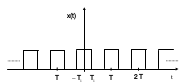
\includegraphics[scale=0.5]{ch10/image1.png}
	\captionof{figure}{Onde carrée périodique}
	\end{wrapfigure}
	Jusqu'à présent, nous n'avons utilisé que des signaux périodiques 
	et l'on voudrait avoir la "généralisation" aux signaux qui ne le
	sont pas. Les coefficients de Fourier de l'onde carrée périodique
	sont :
	\begin{equation}
	a_k = \frac{2\sin(k\omega_0T_1)}{k\omega_0T}
	\end{equation}
	L'idée est de faire tendre la période vers l'infini pour n'en 
	avoir plus qu'une et obtenir un signal apériodique. Le produit
	$Ta_k$ peut être considéré comme un échantillon d'une fonction 
	enveloppe : 
	\begin{equation}
	Ta_k = \frac{2\sin(k\omega_0T_1)}{k\omega_0} = \left.\frac{2\sin
	(\omega T_1)}{\omega}\right|_{\omega=k\omega_0}
	\end{equation}
	En faisant $T\rightarrow\infty$, l'onde carrée devient bien un
	signal apériodique : les coefficients $Ta_k$ tendent vers la 
	fonction \textit{enveloppe}  appelée la \textit{transformée de
	Fourier du signal apériodique.}
	\begin{center}
	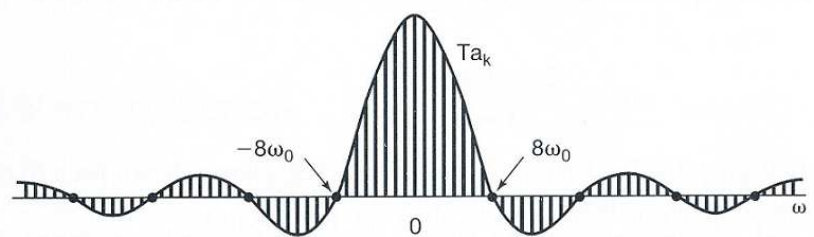
\includegraphics[scale=0.2]{ch10/image2.png}
	\captionof{figure}{Fonction enveloppe}
	\end{center}

		\subsubsection{Généralisation - raisonnement de Joseph Fourier}
		Considérons $x(t)$ t.q. $x(t) =0$ pour $|t|\geq T_1$ et $\tilde{
		x}(t)$ une fonction périodique de période $T$ dont une période 
		coïncide avec $x(t)$.\\
		La série de Fourier de $\tilde{x}(t)$ vaut : 
		\begin{equation}
		\tilde{x}(t) = \sum_{k=-\infty}^\infty a_ke^{ik\omega_0t}\ \ \
		\text{avec }\ \ a_k = \frac{1}{T}\int_{-T/2}^{T/2} \tilde{x}(t)
		e^{-ik\omega_0t}dt
		\end{equation}
		Par définition de $x(t)$ :
		\begin{equation}
		a_k  = \frac{1}{T}\int_{-T/2}^{T/2} x(t)e^{-ik\omega_0t}dt = \frac{1}
		{T}\int_{-\infty}^\infty x(t)e^{-ik\omega_0t}dt
		\end{equation}
		Soit $X(i\omega)$ l'enveloppe de $Ta_k$ :
		\begin{equation}
		X(i\omega) = \int_{-\infty}^\infty x(t)e^{-i\omega t}dt
		\end{equation}
		Il en résulte :
		\begin{equation}
		a_k = \frac{1}{T}X(ik\omega_0)
		\end{equation}
		Soit encore : 
		\begin{equation}
		\begin{array}{ll}
		\tilde{x}(t) &= \sum_{k=-\infty}^\infty \frac{1}{T}X(ik\omega_0)e^
		{ik\omega_0t}\\
		&= \frac{1}{2\pi}\sum_{k=-\infty}^\infty X(ik\omega_0)e^{ik
		\omega_0t}\omega_0
		\end{array}
		\label{eq:ObtFourier}
		\end{equation}
		
		
	\subsection{Transformée de Fourier et transformée inverse}
	\retenir{La (def.) transformée de Fourier est :
	\begin{equation}
	X(i\omega) = \mathcal{F}\{x(t)\} = \int_{-\infty}^\infty x(t)e^
	{-i\omega t}dt
	\end{equation}
	où $X(i\omega)$ est aussi appelé \textit{spectre du signal}.}\ \\
	
	\retenir{La \textbf{transformée de Fourier inverse} s'obtient en 
	faisant 
	tendre $T\rightarrow\infty$ dans \autoref{eq:ObtFourier} :
	\begin{equation}
	x(t) = \mathcal{F}^{-1}\{X(i\omega)\} = \frac{1}{2\pi}\int_{-
	\infty}^\infty X(i\omega)e^{i\omega t} d\omega
	\end{equation}}


	\subsection{Conditions de convergence}
	Il faut en quelque sorte "adapter" les conditions de convergence dans
	le cas de la transformée de Joseph\footnote{Les changements sont 
	mentionnés par un $(!)$.}\footnote{On travaille maintenant dans l'
	espace de carré sommable ou l'expression mathématique de la convergence
	est donnée par $\int_{\infty}^\infty |x(t)|^2dt < \infty$.} :\\
	
	\retenir{\textbf{conditions de Dirichlet}\\
	Les trois conditions de Diriclette s'énoncent :
	\begin{enumerate}
	\item $\int_{-\infty}^\infty |x(t)|\, dt<\infty\ \ \ (!)$
	\item Nombre fini d’extremums dans tout intervalle fini
	\item Nombre fini de discontinuités, uniquement de première espèce,
	dans tout intervalle fini
	\end{enumerate}
	Ces conditions garantissent :
	\begin{itemize}
	\item La convergence de l'intégrale généralisée 
	définissant la transformée de Fourier\ \ \ $(!)$
	\item Égalité entre $x(t)$ et sa série de Fourier en tout point 
	où la fonction est continue.
	\item Aux point de discontinuité de $x(t)\ \ \ (!)$ :
	\begin{equation}
	\frac{x(t^+)+x(t^-)}{2} = \frac{1}{2\pi}\int_{-\infty}^\infty X
	(i\omega)e^{i\omega t}d\omega
	\end{equation}
	\item Tout signal physique admet une transformée de Fourier\ \ \
	$(!)$
	\end{itemize}}\ \\
	
	\exemple{
	\begin{eqnarray}
	X(i\omega) &=&\int_{-\infty}^{+\infty}\overbrace{x(t)}^{e^{-at}\nu(t)}e^{-i\omega t}\,dt=\int_{0}^{+\infty}e^{-(a+i\omega)t}\,dt\\
	 &=& -\frac{1}{a+i\omega}\left[e^{-(a+i\omega)t}\right]_0^{+\infty}
	\end{eqnarray}
	Intéressons-nous a : 
	\begin{equation}
	\lim_{t\rightarrow\infty}\left|e^{-(a+i\omega)t}\right|=\lim_{t\rightarrow\infty}e^{-at}=0\quad\text{car }a>0
	\end{equation}
	Ainsi \begin{equation}
	X(i\omega)=\frac{1}{a+i\omega}
	\end{equation}
	}


\section{Transformée de Fourier d'une fonction périodique continue}
Peut-on calculer la transformée de Fourier d'une fonction périodique 
$x(t)$ à partir de $X(i\omega) = \mathcal{F}\{x(t)\} = \int_{-\infty}
^\infty x(t)e^{-i\omega t}dt$ ?\\
\textbf{Non !} Les fonctions périodiques ne vérifient pas la première 
condition de Dirichlet et ne sont pas de carré sommable : pas possible 
de calculer la transformée de Fourier à partir de l’intégrale généralisée.
Une approche rigoureuse passe par la théorie des distributions, mais nous
ne ferons qu'ici une approche informelle pour énoncer les résultats 
principaux.

	\subsection{Approche informelle}
	Considérons $X(i\omega) = 2\pi\delta(\omega-\omega_0)$. Par la 
	définition de la transformée de Fourier inverse, il vient :
	\begin{equation}
	x(t) = \frac{1}{2\pi}\int_{-\infty}^\infty 2\pi\delta(\omega-
	\omega_0)e^{i\omega t}d\omega = e^{i\omega_0 t}
	\end{equation}
	qui est fonction périodique de période $\frac{2\pi}{\omega_0}$.\\
	Généralisons. Si 
	\begin{equation}
	X(i\omega) = \sum_{-\infty}^\infty 2\pi a_k\delta(\omega-k\omega_0)
	\end{equation}
	alors, par transformée de Fourier inverse,
	\begin{equation}
	x(t) = \frac{1}{2\pi}\int_{-\infty}^\infty \sum_{-\infty}^\infty 2\pi 
	a_k\delta(\omega-k\omega_0)e^{i\omega t}d\omega
	\end{equation}
	Soit
	\begin{equation}
	x(t) = \sum_{-\infty}^\infty a_ke^{ik\omega_0t}
	\end{equation}
	
\section{Propriétés de la transformée de Fourier}
Pour cette section, considérons que la fonction $x(t)$ vérifiant les 
conditions de Dirichlet. La notation pour $x(t)$ et sa transformée de 
Fourier est :
\begin{equation}
x(t) \ft X(i\omega)
\end{equation}

	\subsection{Linéarité}
	Si $x_1(t) \ft X_1(i\omega)$ et $x_2(t) \ft X_2(i\omega)$, alors 
	\begin{equation}
	a_1x_1(t) + a_2x_2(t) \ft a_1X_1(i\omega) + a_2X_2(i\omega)\ \ \
	\forall a_1,a_2 \in \mathbb{C}
	\end{equation}
	
	\subsection{Propriétés de symétrie}
		\subsubsection{Première propriété}
		Si $x(t) \ft X(i\omega)$, alors
		\begin{equation}
		\overline{x}(t) \ft \overline{X}(-i\omega)
		\end{equation}	
		\begin{proof}\ \\
		Calculons le conjugué suivant :
		\begin{equation}
		\overline{X}(i\omega) = \overline{\int_{-\infty}^\infty x(t)e^{-
		i\omega t}dt} = \int_{-\infty}^\infty \overline{x}(t)e^{i\omega t}dt
		\end{equation}	
		En remplaçant $\omega$ par $-\omega$ :
		\begin{equation}
		\overline{X}(-i\omega) = \int_{-\infty}^\infty \overline{x}(t)e^{-i
		\omega t}dt = \mathcal{F}(\overline{x}(t))
		\end{equation}
		\end{proof}
	
		\subsubsection{Deuxième propriété}
		Si $x(t) \ft X(i\omega)$ et $x(t)$ est réelle, alors 	
		\begin{equation}
		\overline{X}(i\omega) = X(-i\omega)
		\end{equation}
		La transformée de Fourier $X(i\omega)$ est une fonction paire.
	
		\subsubsection{Troisième propriété}
		L'expression de $X(i\omega)$ en coordonnées cartésiennes est : 
		\begin{equation}
		X(i\omega) = \Re(X(i\omega)) + i\Im(X(i\omega))
		\end{equation}
		Si $x(t)$ est réelle :
		\begin{equation}
		\begin{array}{ll}
		\overline{X}(i\omega) &= \Re(X(i\omega))-i\Im
		(X(i\omega))\\
		&= \Re(X(-i\omega)) + \Im(X(-i\omega))
		\end{array}
		\end{equation}
		Ceci implique que $\Re(X(i\omega))$ est une fonction 
		\textbf{paire} et $\Im(X(i\omega))$ une fonction 
		\textbf{impaire}.
	
	
		\subsubsection{Quatrième propriété}
		L'expression de $X(i\omega)$ en coordonnées polaire est : 
		\begin{equation}
		X(i\omega) = |X(i\omega)|e^{i\varphi(\omega)}
		\end{equation}
		Toujours pour un signal $x(t)$ réel :
		\begin{equation}
		\begin{array}{ll}
		\overline{X}(i\omega) &= |X(i\omega)|e^{-i\varphi(\omega)}\\
		 &= |X(-i\omega)|e^{i\varphi(-\omega)}
		\end{array}
		\end{equation}
		Ceci implique que $|X(i\omega)|$ est une fonction \textbf{paire} 
		et $\varphi(\omega)$ une fonction \textbf{impaire}.
		
	
		\subsubsection{Cinquième propriété}
		Si $x(t)$ est une fonction réelle et \textbf{paire}, alors $X(i
		\omega)$ est réelle et paire.\\
		Si $x(t)$ est une fonction réelle et \textbf{impaire}, alors 
		$X(i\omega)$ est purement imaginaire et impaire.
		
	\subsection{Glissement dans le temps}
	Si $x(t) \ft X(i\omega)$, alors 
	\begin{equation}
	x(t-t_0) \ft e^{-i\omega t_0}X(i\omega)
	\end{equation}
	Ceci résulte de 
	\begin{equation}
	\begin{array}{ll}
	\mathcal{F}(x(t-t_0)) &= \int_{-\infty}^\infty x(t-t_0)e^{-i\omega t}dt\\
	&= e^{-i\omega t_0} \int_{-\infty}^\infty x(\tau)e^{-i\omega\tau}d\tau \\
	&= e^{-i\omega t_0}X(i\omega)
	\end{array}
	\end{equation}
	Ceci signifie qu'un glissement temporel subi par $x(t)$ correspond à un 
	déphasage de $-\omega t_0$ dans la transformée de Fourier (et aucun 
	changement du module $|X(i\omega)|$).
	
	\subsection{Glissement en fréquence}
	Si $x(t) \ft X(i\omega)$, alors 
	\begin{equation}
	e^{i\omega_0t}x(t) \ft X(i(\omega-\omega_0))
	\end{equation}
	On observe ici une dualité entre glissement temporel et glissement 
	en fréquence.\\
	
	\exemple{
	\begin{eqnarray}
	x(t)\cos(\omega_0t) &=& x(t)\frac{e^{i\omega t}+e^{-i\omega t}}{2}\\
	x(t)\cos(\omega_0t) &\Leftrightarrow&\frac{1}{2}\left[X(i(\omega-\omega_0))+X(i(\omega+\omega_0))\right]
	\end{eqnarray}
	}
	
	\subsection{Changement d'échelle}
	Si $x(t) \ft X(i\omega)$, alors 
	\begin{equation}
	x(at) \ft \frac{1}{|a|}X\left(i\frac{\omega}{a}\right)\ \ a\in\mathbb{R}
	_0
	\end{equation}
	Ceci s'obtient par changement de variable $q=at$. Cela signifie qu'une 
	compression/dilatation du temps $\Leftrightarrow$ dilatation/compression 
	en fréquence.

	\subsection{Transformée de Fourier de la dérivée d'une fonction}
	Si $x(t) \ft X(i\omega)$ et si $\frac{dx(t)}{dt}$ vérifie les conditions
	de Dirichlet, alors
	\begin{equation}
	\frac{dx(t)}{dt} \ft i\omega X(i\omega)
	\end{equation}
	Ceci permet de changer une dérivation en une multiplication algébrique (
	Oh, les phaseurs!).\\
	Ce résultat s'obtient en intégrant par partie :
	\begin{equation}
	\begin{array}{ll}
	\mathcal{F}\left(\frac{dx(t)}{dt}\right) &= \int_{-\infty}^\infty \frac{dx(t)}
	{dt}e^{-i\omega t}dt\\
	 &= \left.x(t)e^{-i\omega t}\right|_{-\infty}^\infty - \int_{-\infty}^\infty x(t)
	 \frac{d}{dt}e^{-i\omega t}dt\\
	 &= \left.x(t)e^{-i\omega t}\right|_{-\infty}^\infty +i\omega \int_{-\infty}^
	 \infty x(t)e^{-i\omega t}dt\\
	\end{array}
	\end{equation}
	Le premier s'annule par les conditions de Dirichlet (hypothèse) et on retrouve 
	bien le résultat.
		
	\subsection{Dérivée de la transformée de Fourier}
	Si $x(t) \ft X(i\omega)$ et $tx(t)$ vérifie les conditions de Dirichlet,
	alors:
	\begin{equation}
	-itx(t) \ft \frac{dX(i\omega)}{d\omega}
	\end{equation}
	Ceci résulte de :
	\begin{equation}
	\begin{array}{ll}
	\frac{dX(i\omega)}{d\omega} &= \frac{d}{d\omega}\int_{-\infty}^\infty 
	x(t)e^{-i\omega t}dt\\
	 &= -i \int_{-\infty}^\infty tx(t)e^{-i\omega t}dt = -i\mathcal{F}\{tx(t)\}
	\end{array}
	\end{equation}



	\subsection{Transformée de Fourier d'une convolution}
	Il s'agit d'une règle fondamentale ! \textit{La démonstration est très sympathique
	pour l'examen, courte et simple à corriger.}\\
	Soit $s(t) \ft S(i\omega)$ et $q(t) \ft Q(i\omega)$. Si $s(t)*q(t)$ vérifie les 
	conditions de Dirichlet, alors :
	\begin{equation}
	x(t) = s(t)*q(t) \ft X(i\omega) = S(i\omega)Q(i\omega)
	\label{eq:TransfoConvol}
	\end{equation}
	Le produit de \textbf{convolution} devient produit \textbf{algébrique} par transformée 
	de Fourier.
	
	\begin{proof}\ \\
	Partons de l'expression de la transformée de Fourier :
	\begin{equation}
	X(i\omega) = \int_{-\infty}^\infty x(t)e^{-i\omega t}dt
	\label{eq:DebutDemo}
	\end{equation}
	En appliquant la définition du produit de convolution :
	\begin{equation}
	X(i\omega) = \int_{-\infty}^\infty \left[\int_{-\infty}^\infty s(\tau)q(t-\tau)d\tau
	\right]e^{-i\omega t}dt
	\end{equation}
	En regroupant tout ce qui fait intervenir le temps :
	\begin{equation}
	X(i\omega) = \int_{-\infty}^\infty s(\tau)\left[\int_{-\infty}^\infty q(t-\tau)e^{-i
	\omega t}dt\right]d\tau
	\end{equation}
	On voit apparaître l'expression de la transformée de Fourier translatée dans le temps. En
	appliquant la règle de glissement dans le temps : 
	\begin{equation}
	Q(i\omega)e^{-i\omega \tau} = \int_{-\infty}^\infty q(t-\tau)e^{-i\omega t}dt
	\end{equation}
	Après substitution dans \autoref{eq:DebutDemo} :
	\begin{equation}
	X(i\omega) = \int_{-\infty}^\infty s(\tau)Q(i\omega)e^{-i\omega\tau}d\tau = S(i\omega)Q(i
	\omega)
	\end{equation}
	\end{proof}
	
	\subsection{Transformée de Fourier d'un produit}
	Soit $s(t) \ft S(i\omega)$ et $q(t) \ft Q(i\omega)$. Supposons que $r(t) = s(t)q(t)$ 
	vérifie les conditions de Dirichlet. La transformation d'un produit algébrique simple 
	va donner un produit de \textbf{convolution}, à un facteur près :
	\begin{equation}
	r(t) = s(t)q(t) \ft R(i\omega) = \frac{1}{2\pi}(S(i\omega)*Q(i\omega))
	\end{equation}
	
	\begin{proof}\ \\
	La démonstration est très semblable à la dernière. Il faut cependant veiller à faire un 
	changement de variable (par exemple $\theta$) pour ne pas confondre les $\omega$\footnote{
	Erreur fréquente à l'examen.}. Voir slide 50/55 dont voici les "clés de la démos :
	\begin{itemize}
	\item On applique la transformée inverse avec le facteur $1/2\pi$.
	\item Il faut intervertir l'ordre d'intégration et regrouper tout ce qui dépend de $t$
	\item On voit alors apparaître la définition de la transformée de Fourier où  $\omega$
	est remplacé par $\omega-\theta$ : on retrouve l'expression de la convolution.
	\end{itemize}
	\end{proof}
	
	
	
	\subsection{Relation de Parceval (ou théorème de Plancherel)}	
	Si $X(i\omega) \ft \mathcal{F}(x(t))$, alors 
	\begin{equation}
	\int_{-\infty}^\infty |x(t)|^2 dt = \frac{1}{2\pi}\int_{-\infty}^\infty |X(i\omega)|^2
	d\omega
	\end{equation}
	Cette relation permet de calculer l'énergie totale d'un signal à partir de son spectre.
	
	\begin{proof}\ \\
	Vue en cours ? J'sais plus :( Slide 55/55).
	\end{proof}
	
	
	
	
	
	
	
	
	
	
	
	
	
	
	
	
	
	
	
	
	
	
	
	
	
	
	
	
	
	
	
	
	
	
	
	
